% !TeX root = ../thuthesis-example.tex

\chapter{总结}
\thusetup{
  cite-style = super,
}
\section{本文结论}
本文依照优化技术归纳、同类算子演绎和编译算法设计的思路展示了针对稀疏稠密混合代数在单指令多线程架构上灵活规约优化空间扩展的编译算法设计,在算子性能、优化技术泛化性和开发效率方面取得了提升,并为更广泛的通用稀疏张量计算编译算法设计提出了可行的研究方法。
针对稀疏稠密混合代数在SIMT架构上优化不充分和开发难度高的问题,本文提出了灵活规约优化技术和灵活规约语义提升技术。

灵活规约优化技术包含灵活规约粒度和规约策略,该技术扩展了当前的基于原子并行模型的稀疏稠密混合代数优化空间。同时本文从张量形式和表形式两个角度论证了在原理上可以将性能提升泛化至所有稀疏稠密混合代数。
实验结果显示,在稀疏稠密矩阵向量乘算子上灵活规约取得了比最优开源算子库1.6到2.7倍性能提升。

基于扩展后的优化空间,本文将灵活规约纳入稀疏迭代模型,并提出灵活规约语义提升技术,在稀疏算子编译器前端添加灵活规约调度参数;中端添加并行规约数据流;后端添加高效规约模板。
该技术使得用户可以通过简单调度指令针对任意稀疏稠密混合代数进行灵活规约扩展优化空间的性能调优。实验结果显示,该技术将原有稀疏算子编译器生成的SpMM性能提升平均1.2倍,最高3.8倍;MTTKRP算子最高提升2.7倍。


\section{相关工作}
下面首先回顾算子编译器产生动机,指出其学术研究价值和产业应用潜力。张量编译器指为高效张量计算设计的编译器\cite{halide,kjolstad:2017:taco}。常见的张量编译器输入为描述张量运算的高级语言。
深度学习编译器\cite{tvm,rammer}的核心之一也是张量编译器,因为当前机器学习算法的核心算子为张量运算。常见深度学习编译器输入为神经网络计算图描述语言和参数文件。
二者输出均为硬件平台特定低级语言。与张量编译器不同,深度学习编译器同时还包含计算图优化,算子融合等技术。因为二者技术类似,所以下面统称算子编译器。
深度学习框架\cite{tensorflow,pytorch}与算子编译器不同。框架常以扩展包形式嵌入到其他常用高级语言(如Python, C++),不直接输出硬件算子,而是调用硬件平台提供的算子库(如英伟达GPU的cuDNN算子库\cite{cuDNN})。
算子编译器较算子库相比优势为开发成本低和灵活度高。在实际生产中,针对特定硬件的高效深度学习算子库开发长达几个月甚至几年,很难满足专用硬件量产需求和算法迭代速度\cite{Heron}。
而编译器可以通过计算元语模板和优化空间自动探索技术,在几小时甚至几分钟内生成和算子库性能相当的算子\cite{Roller}。同时,因为编译器可以做代码级别变换,所以很方便做算子融合。
算子融合技术可以加速深度学习算法推理速度,最高可达10倍左右\cite{DNNFusion}。而算子库的功能在开发时就已确定,无法做细粒度的算子融合\cite{Graphene}。
因此,有越来越多学者开始关注这一领域\cite{PET,Tiramisu,Checkmate},硬件提供商也在积极研发算子编译器技术,比如英伟达的Triton\cite{Triton},和华为的AKG\cite{AKG}。

\section{未来工作}
上节分析了算子编译器的发展动机,下面基于三个典型问题阐释算子编译器的核心优化技术,并指出未来可能的研究和应用方向。

第一个问题:算子编译器能否表达手工算子优化的技术?硬件架构特性规定了所有可能的算子优化技术。以GPU为例,double-buffer技术基于GPU的shared memory-register file两层级存储架构\cite{double-buffer};并行规约技术基于GPU的CUDA Core中线程同步架构\cite{parallel-reduction};
tiling技术基于DRAM的coalesce访存架构\cite{coalesce};data-layout在寄存器中的排布要适应Tensor Core的指令特殊规定\cite{DynamicNM}。因此,如果算子编译器
生成的算子想要逼近甚至超过算子库性能,算子编译器就需要可以表达尽可能多的手工算子优化技术。这是算子编译器的基本问题,因为如果无法表达算子优化技术,无论怎么微调参数都难以超过手工算子性能。
换句话讲,算子编译器需要随着硬件架构的演进不断扩展优化空间。因此,只要应用需求推动硬件架构持续创新,算子编译器领域就将大概率出现更多新技术。

已有较多工作基于此思路。比如ALCOP\cite{ALCOP}基于Tensor Core架构将“多级访存-计算流水线”算子技术引入算子编译器,生成的算子较TVM1.23倍的平均加速;
TensorIR\cite{TensorIR}基于Tensor Core架构引入硬件特殊加速的特定形状矩阵乘法,生成的算子较TVM提升了最多7.5倍。 本文也是沿着这个思路。
首先通过分析GPU架构特征,提出灵活规约同步粒度这一稀疏稠密混合算子优化技术。手工验证该技术有效后,通过在后端设计算子模版,中端调整计算流图,前端设计调度API,最终实现用户仅添加一条调度指令就可以享受到算子性能提升。

第二个问题:如何设计中间表示(intermediate representation,简称IR)?IR是连接用户代码和机器码的中间组件\cite{IR},它是编译器表达手工算子优化技术的手段。如果没有IR,即用户代码直接经过多次变换生成机器码,会有两个问题:部署成本高和维护复杂。机器的ISA更改则必须重写编译器,由于前端后端强耦合,更改编译器代码会产生副作用\cite{LLVM}。
因此,算子编译器也需要IR。算子编译器中有三类常见IR:一是顶层抽象编译器支持的操作,二是底层抽象硬件架构,三是中层连接性的IR。底层IR为顶层IR提供计算平台基础,顶层IR为底层IR提供应用场景,中层IR作为编译变换的载体连接底层和顶层IR。

从硬件角度设计底层IR比如,在TVM\cite{tvm}中,GPU的并行计算单元被抽象为二维blockIdx和二维threadIdx;而在Roller\cite{Roller}中单个计算单元的能力被抽象为load, compute, store,GPU则被抽象为大量相同的该计算单元;也可以借助MLIR提供的层次化编译变换提供GPU Tensor Core的硬件抽象\cite{mlir-tc}。
从应用角度设计顶层IR比如,CoRA\cite{CoRA}针对不规则稠密矩阵应用设计IR来更高效地规则化计算和融合算子;SparseTIR\cite{SparseTIR}针对稀疏张量计算设计IR来表示数据格式融合和高效混合计算。
当然,也可以先从应用角度设计顶层IR,然后直接将顶层IR中的关键操作设置为底层IR,根据底层IR设计新的硬件架构。比如,SAM\cite{SAM}抽象出稀疏张量运算的9种核心操作,并为稀疏张量数据流加速器提供了直接的硬件模块映射。

第三个问题:算子编译器算子生成效率?由于算子编译器较算子库的一大优势是开发成本低,因此如何更快生成好算子是一个重要的研究问题。这一问题包含两方面:快速判断一个算子的质量(即在实际硬件上运行的速度)和快速生成优质算子。
算子质量判断有两种主流方向。一种是基于搜索得到算子的实际性能历史记录学习得到的机器学习模型,另一种是基于架构特征的近似解析模型。机器学习模型的优势是算法设计和硬件无关,容易迁移;但劣势是需要积累实测的历史数据,搜索时间较长且可解释性差\cite{AutoTVM,Ansor,AMOS}。
解析模型的优势是不需要实测历史记录,可解释性强,但劣势是和架构相关,且需要基于一定假设才能得到近似,容易出现估计偏差\cite{GNNAdvisor,Roller,ALCOP}。
快速生成优质算子常见算法是基于给定元语集合的遗传算法和基于手写模板的快速参数搜索算法。遗传算法的优势是可以探索人工设计没有考虑到的元语组合,劣势是搜索空间稀疏,难以快速搜索到优质算子\cite{Hidet}。
基于手写模板的参数搜索算法优势是可以较快探索局部优化空间,劣势是优化空间受限\cite{Auto-Halide}。

由于稀疏计算复杂性,其优化空间构建仍是开放问题。与稠密计算不同,稀疏计算涉及坐标空间和位置空间变换,而稠密计算一直在坐标空间,这进一步加剧了优化空间的稀疏性\cite{senanayake:2020:scheduling}。
同时稀疏计算任务规模在运行前不可知,而稠密计算可以在运行前分析输入数据并做优化,这对算子编译器运行时优化提出了更大的挑战\cite{Dynamic-tiling}。
因此,当前提升稀疏算子编译器算子生成效率的研究仍处于基于手写模板的阶段。比如TACO自动调度\cite{ahrens:2022:autoscheduling}基于最小化冗余计算的原理提出了构建渐进复杂度意义下最优算子的原则,
WACO\cite{WACO}基于TACO\cite{kjolstad:2017:taco}提供的元语,为稀疏稠密混合代数设计了算子模板,离线构造优化空间,运行时根据输入数据特征搜索最优解。

总的来说,算子开发的目标是更高性能和更高迭代效率,相关技术发展有三大趋势:自动化,结构化和智能化,如图~\ref{fig:future}所示。自动化是指将已经确定的代码写法固化为模板,由程序自动生成。比如本文编译算法的宏指令设计就是将灵活规约固化为模板,有编译器中端自动调用。在实际应用中,英伟达采用模板编程开发了高效线性代数库CUTLASS\cite{CUTLASS}。
该种方式最直接,但是不灵活。结构化是指将已有的优化技术通过中间表示泛化至一类算子。比如本文编译算法的标量转移空间设计就是将灵活规约通过LLIR应用到所有稀疏稠密混合代数中。在实际应用中,Halide\cite{halide},TVM\cite{tvm}和TACO\cite{kjolstad:2017:taco}都采用了该种技术。该种技术一定程度上降低了优化技巧泛化成本,但是优化空间仍然
限制在人工经验中。智能化是指利用基础模型\cite{Bommasani2021FoundationModels}学习优化技术直接生成算子。这种技术难点是构建反馈闭环,将算子建模为基础模型的序列化输入,以及人工经验的合理嵌入。该种方案可以突破人工经验,迈向算子极致性能优化。
\begin{figure}
  \centering
  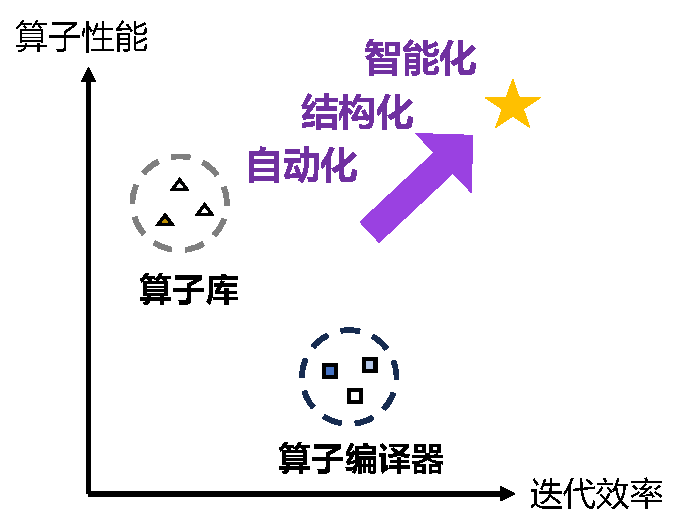
\includegraphics[width=0.6\linewidth]{future.pdf}
  \caption{算子优化技术发展趋势}
  \label{fig:future}
\end{figure}